%%%%%% CMB-S4 Neutrinos Chapter  %%%%%%%%%%%%%%%%
 
\chapter{Neutrino Physics from the Cosmic Microwave Background}
\renewcommand*\thesection{\arabic{section}}

\def\beq{\begin{equation}}
\def\eeq{\end{equation}}

\def\bea{\begin{eqnarray}}
\def\eea{\end{eqnarray}}

\def\Neff{N_{\rm eff}}
\def\gtrsim{\raise-.75ex\hbox{$\buildrel>\over\sim$}}
%%%%%%%%%%%%%%%%%%%%%%%%%%%%%%%%%%%%%%%%%%%%%%%%%%%%%%%%%%%
%%%%%%%%%%%%%%%%%%%%%%%%%%%%%%%%%%%%%%%%%%%%%%%%%%%%%%%%%%%
%%%%%%%%%%%%%%%%%%%%%%%%%%%%%%%%%%%%%%%%%%%%%%%%%%%%%%%%%%%
%%%%%%%%%%%%%%%%%%%%%%%%%%%%%%%%%%%%%%%%%%%%%%%%%%%%%%%%%%%

\section{Introduction}

Direct interactions between neutrinos and observable matter effectively ceased about one second after the end of inflation.  Nevertheless, the total energy density carried by neutrinos was comparable to other matter sources through today.  As a result, the gravitational effect of the neutrinos is detectable both at the time of recombination and in the growth of structure at later times~\cite{Abazajian:2013oma}, leaving imprints in the temperature and polarization spectrum as well as in CMB lensing.

CMB-S4 can improve our understanding of neutrino physics in regimes of interest for both cosmology and particle physics.  Arguably the most important parameters of interest will be the sum of the neutrino masses $\sum m_\nu$ and the effective number of neutrino species, $\Neff$.  These two parameters have natural targets that are within reach of a CMB-S4 experiment:
\begin{itemize}
\item $ \sum m_\nu \gtrsim 58$ meV is the lower bound guaranteed by observations of solar and atmospheric neutrino oscillations.  A CMB experiment with $\sigma(\sum m_\nu) < 20$ meV would be guaranteed a detection of a least 3$\sigma$.
\item $\Delta \Neff > 0.027$ is predicted for any light particle that was in thermal equilibrium with the standard model.  A CMB experiment producing $\sigma(\Neff) \lesssim 0.01$ would be sensitive to all models in this very broad class of extensions of the Standard Model, which includes a wide range of axions and axion-like particles.  
\end{itemize}
Current CMB data already provides a robust detection of the cosmic neutrino background at $>10 \sigma$.  A CMB-S4 experiment will provide an order of magnitude improvement in sensitivity that opens a new window back to the time of neutrino decoupling and beyond.

Section 2 will review the motivation for studying neutrino masses with cosmological probes, and specifically with the CMB.  We will explain why cosmology is sensitive to $\sum m_\nu$ via different probes and how it is complementary to the experimental neutrino effort.  Section 3 will review the physics of $\Neff$ and its role as probe of the C$\nu$B and as sensitive tool for beyond the Standard model physics.  We will emphasize the unique impact $\Neff$ has on the CMB that makes it distinguishable from other extensions of $\Lambda$CDM.  In Section 4 we will discuss the implications for a variety of well motivated models, including sterile neutrinos and axions.   

\section{Neutrino Mass}

\subsection{Theory Review}

{\it Subsection to be completed by Marilena Loverde}



\subsection{Observational Signatures and Target}

Massive neutrinos contribute to the critical density as
\beq
\Omega_\nu h^2 \simeq \frac{\sum m_\nu}{93 \, {\rm eV}} \ .
\eeq

\subsubsection{CMB Power Spectra (TT, EE, Lensing Potential)}

\subsubsection{SZ Cluster Abundance}

\subsubsection{Cross-correlations with External Datasets}


\subsection{Forecasts}

\subsection{Relation to Lab Experiments}

Relation between lab measurements of neutrino masses and the cosmological measurements.

\section{Effective Number of Neutrinos}

\subsection{Theory Review}

{\it Subsection to be completed by Joel Meyers with a contribution from George Fuller}

The {\it effective} number of neutrinos defined to be
\beq
\Neff=\frac{8}{7} \left(\frac{11}{4}\right)^{4/3} \frac{\rho_{R}-\rho_\gamma}{\rho_\gamma}  \ ,
\eeq
where $\rho_{R}$ is the total energy density in radiation and $\rho_\gamma$ is the energy density in photons. 

{\it Status of calculations in the Standard Model} -- (Contribution expected from G. Fuller)


{\it Light Species}

\begin{figure}[t!]
\begin{center}
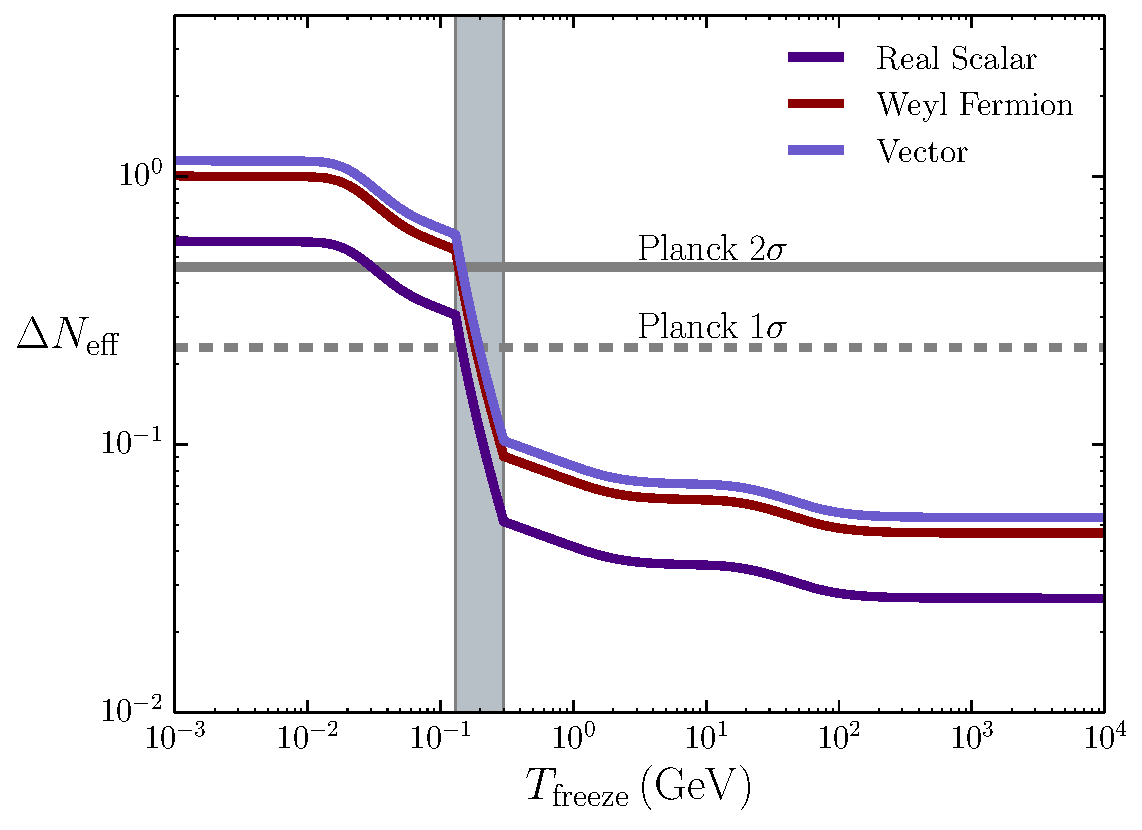
\includegraphics[width=0.65\textwidth]{Neutrinos/Neff.pdf}
\caption{Contribution to $\Neff$ from a massless field that was in thermal equilibrium with the Standard model at temperatures $T> T_{\rm freeze}$.  For $T_{\rm freeze} \gg m_{\rm top}$, these curves saturate with $\Delta \Neff > 0.027$.   The region in red shows the range of forecasts for $\sigma(\Neff)$ for plausible CMB-S4 configurations. }
\label{fig:limits}
\end{center}
\end{figure}

\subsection{Observational Signatures}

Cosmic neutrinos play to two important roles in the CMB that are measured by $\Neff$.  They contribute to the total energy in radiation which controls the expansion history and, indirectly, the damping tail.  The fluctuations of neutrinos and any other free streaming radiation also produces a constant shift in the of the acoustic peaks.  These two effects drive both current and future constraints on $\Neff$.  

The effect of neutrinos on the damping tail has dominated has historically driven the constraint on $\Neff$ in the CMB.  The largest effect is from the mean-free path of photons, which introduces a suppression $e^{-(k/k_d)^2}$ to short wavelengths, with~\cite{Zaldarriaga:1995gi}
\beq
k_d^{-2} =\int \frac{da}{a^3 \sigma_T n_e H} \frac{R^2+ \frac{16}{15}(1+R)}{6(1+R)^2} \ ,
\eeq
where $R$ is the ratio of the energy in baryons to photons, $n_e$ is the density of free electrons and $\sigma_T$ is the Thompson cross-section.  The damping scale is sensitive to the energy in all radiation through $H \propto \sqrt{\rho_{\rm radiation}}$ during radiation domination (which is applicable at high $\ell$, and is therefore sensitive to $\Neff$ or any form of dark radiation.  At this level, this also illustrates the degeneracy with $n_e$ which may be altered by the helium fraction, $Y_p$.

In reality, the effect on the damping tail is actually subdominant to the change to the scale of matter radiation equality and the location of the first acoustic peak~\cite{Hou:2011ec}.  As a result, the effect on neutrinos on the damping tail is more accurately represented by holding the first acoustic peak fixed.  This changes the sign of the effect on the damping tail, but the intuition for the origin of the effect (and degeneracy) remain applicable.

In addition to the effect on the Hubble expansion, perturbations in neutrinos effect the photon-baryon fluid through their gravitational influence.  The contributions from neutrinos are well described by a correction to the amplitude and the phase of the acoustic peaks in both temperature and polarization~\cite{Bashinsky:2003tk}.  The phase shift is a particularly compelling signature as it is not degenerate with other cosmological parameters~\cite{Bashinsky:2003tk,Baumann:2015rya}.  This effect is the result of the free-streaming nature of neutrinos that allows propagation speeds of effectively the speed of light (while the neutrinos are relativistic).  This effect is sensitive to any gravitationally coupled light thermal relics.

E-mode polarization will play an increasingly important role for several reasons.  First of all, the acoustic peaks are sharper in polarization which makes measurements of the peak locations more precise, and therefore aid the measurement of the phase shift.  The second reason is that polarization breaks a number of degeneracies that would also affect the damping tail~\cite{Baumann:2015rya}.

{\it Status of current observations} -- Planck has provided a strong constraint on $\Neff = 3.15 \pm 0.23$ when combining both temperature and polarization data.  The addition of polarization data has both improved the constraint on $\Neff$ and reduced the impact of the degeneracy with $Y_p$.  Recently, the phase shift from neutrinos has also been established direction in the Planck temperature data~\cite{Follin:2015hya}.  This provides the most direct evidence for presence of free-steaming radiation in the early universe, consistent with the cosmic neutrino background.


\subsection{Forecasts}

\subsection{Thermal History and Big Bang Nucleosynthesis}

{\it Subsection to be completed by Joel Meyers}



\section{Sterile Neutrinos and Other Targets}
\subsection{Sterile Neutrinos}

{\it Subsection to be completed by Kevork Abazajian}

\subsection{Axion-like Particles}

{\it Subsection to be completed by Dan Green}

\subsection{Energy Injection and Particle Decays}

\subsection{Connections to BBN and Spectral Distortions}


\bibliography{cmbs4}

%%
%% Populate the .bib file with entries from SPIRES Bibtex (preferred)
%% or ADS Bibtex (if no SPIRES entry).
%%  SPIRES will also supply the CITATION line information; please include it.
%%


